\PassOptionsToPackage{unicode=true}{hyperref} % options for packages loaded elsewhere
\PassOptionsToPackage{hyphens}{url}
%
\documentclass[]{article}
\usepackage{stata}
\usepackage{lmodern}
\usepackage{amssymb,amsmath}
\usepackage{ifxetex,ifluatex}
\usepackage{fixltx2e} % provides \textsubscript
\ifnum 0\ifxetex 1\fi\ifluatex 1\fi=0 % if pdftex
  \usepackage[T1]{fontenc}
  \usepackage[utf8]{inputenc}
  \usepackage{textcomp} % provides euro and other symbols
\else % if luatex or xelatex
  \usepackage{unicode-math}
  \defaultfontfeatures{Ligatures=TeX,Scale=MatchLowercase}
\fi
% use upquote if available, for straight quotes in verbatim environments
\IfFileExists{upquote.sty}{\usepackage{upquote}}{}
% use microtype if available
\IfFileExists{microtype.sty}{%
\usepackage[]{microtype}
\UseMicrotypeSet[protrusion]{basicmath} % disable protrusion for tt fonts
}{}
\IfFileExists{parskip.sty}{%
\usepackage{parskip}
}{% else
\setlength{\parindent}{0pt}
\setlength{\parskip}{6pt plus 2pt minus 1pt}
}
\usepackage{hyperref}
\hypersetup{
            pdftitle={Stata Markdown Tutorial},
            pdfauthor={Cyrus Samii},
            pdfborder={0 0 0},
            breaklinks=true}
\urlstyle{same}  % don't use monospace font for urls
\usepackage{graphicx,grffile}
\makeatletter
\def\maxwidth{\ifdim\Gin@nat@width>\linewidth\linewidth\else\Gin@nat@width\fi}
\def\maxheight{\ifdim\Gin@nat@height>\textheight\textheight\else\Gin@nat@height\fi}
\makeatother
% Scale images if necessary, so that they will not overflow the page
% margins by default, and it is still possible to overwrite the defaults
% using explicit options in \includegraphics[width, height, ...]{}
\setkeys{Gin}{width=\maxwidth,height=\maxheight,keepaspectratio}
\setlength{\emergencystretch}{3em}  % prevent overfull lines
\providecommand{\tightlist}{%
  \setlength{\itemsep}{0pt}\setlength{\parskip}{0pt}}
\setcounter{secnumdepth}{0}
% Redefines (sub)paragraphs to behave more like sections
\ifx\paragraph\undefined\else
\let\oldparagraph\paragraph
\renewcommand{\paragraph}[1]{\oldparagraph{#1}\mbox{}}
\fi
\ifx\subparagraph\undefined\else
\let\oldsubparagraph\subparagraph
\renewcommand{\subparagraph}[1]{\oldsubparagraph{#1}\mbox{}}
\fi

% set default figure placement to htbp
\makeatletter
\def\fps@figure{htbp}
\makeatother

\usepackage{multicol}
\usepackage{tabularx}
\usepackage{booktabs}
\usepackage{lscape}
\usepackage{fullpage}
\usepackage{pgffor}

\title{Stata Markdown Tutorial}
\author{Cyrus Samii}
\date{January 2019}

\begin{document}
\maketitle

\hypertarget{overview}{%
\section{Overview}\label{overview}}

Here are some notes and examples for using the Stata Markdown package.
The Stata Markdown package was written by German Rodriguez. These notes
offer some basic guidance on using the package. For instructions on
installation and dependencies, refer to the Stata Markdown website:

\url{https://data.princeton.edu/stata/markdown/}

I give examples of some things we might want to do in social science
related projects.

\hypertarget{markdown}{%
\section{Markdown}\label{markdown}}

Markdown is a simple markup language that, through Pandoc, can be
rendered in a variety of formats, including pdf (via tex), html, or
docx.\\
If you are used to writing latex or html, then markdown will be easy,
since it admits a lot of the syntax used in those languages.

There are lots of cheatsheets out there, such as:

\url{https://github.com/adam-p/markdown-here/wiki/Markdown-Cheatsheet}

Lots of things are done very simply in Markdown. E.g., here is a
numbered list:

\begin{enumerate}
\def\labelenumi{\arabic{enumi}.}
\tightlist
\item
  Foo
\item
  Foo 2
\item
  Foo 3
\end{enumerate}

The header of this document is a YAML header for Markdown, which
contains meta instructions for the Markdown-\textgreater{}Pandoc
compilation. I am rendering this document in PDF through Tex, and so you
will see that in my YAML header I have included some Tex instructions.

\hypertarget{workflow}{%
\section{Workflow}\label{workflow}}

The way I work is to type into this document and then compile by running
the requisite commands that I have put into a separate .do file called
``stata-markdown-example-do.do''. That way, I can load the various
compilation options (that is, the options to the \texttt{markstat}
function in a way that I can easily recall them later. Using the
\texttt{do} button in the Stata .do file editor gives me one button
compilation. I also have my commands to set the working directory and
also load in dependencies (e.g., the \texttt{stata.sty} file needed to
compile to PDF).

I may also have another Stata .do file that I use as a scratch pad for
working out the kinks of the Stata code that I then insert as code
chunks into this document.

\hypertarget{simple-script-example}{%
\section{``Simple Script'' Example}\label{simple-script-example}}

Here we replicate the simple example from German Rodriguez's ``Simple
Script'' example, tweaking a few things to make some additional points.

Stata code appears below in ``chunks'' that are demarcated in the
following manner:

For code chunks that you want to appear in the rendered document:

\begin{verbatim}```{s} 
[code here] 
```
\end{verbatim}

For code chunks that you DO NOT want to appear in the rendered document:

\begin{verbatim}```{s/} 
[code here] 
```
\end{verbatim}

Now we can proceed with the simple example. First read in the fuel
efficiency data that is shipped with Stata:

\begin{stlog}
. sysuse auto, clear
(1978 Automobile Data)
\end{stlog}

To study how fuel efficiency depends on weight it is useful to transform
the dependent variable from ``miles per gallon'' to ``gallons per 100
miles'':

\begin{stlog}
. gen gphm = 100/mpg
\end{stlog}

We can then plot the relationship. We will run this code in a manner
that is not echoed in the resulting output file (PDF, docx, etc.).

\begin{stlog}


{\smallskip}

\end{stlog}

\begin{figure}
\centering
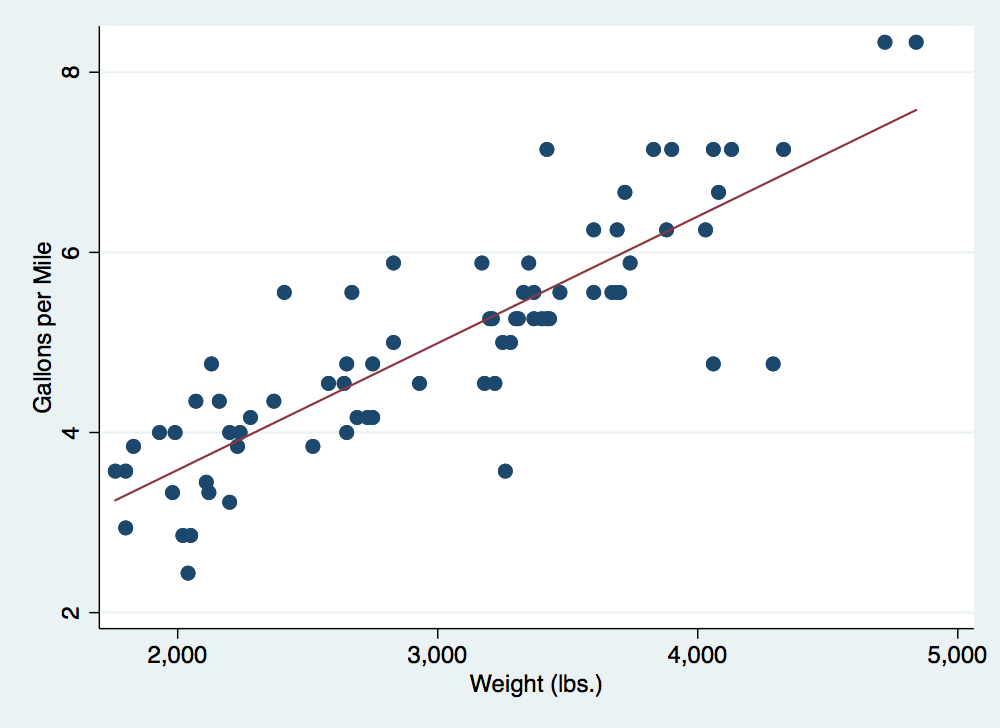
\includegraphics[width=0.75\linewidth]{auto.png}
\caption{Fuel Efficiency}
\end{figure}

\hypertarget{regression-table-with-esttab}{%
\section{\texorpdfstring{Regression table with
\texttt{esttab}}{Regression table with esttab}}\label{regression-table-with-esttab}}

Something that we frequently need to do is to report regression tables.
We can use the \texttt{esttab} function in Stata and insert its output
here:

\begin{stlog}

{\smallskip}

{\smallskip}


\end{stlog}

\begin{center}
{
\def\sym#1{\ifmmode^{#1}\else\(^{#1}\)\fi}
\begin{tabular}{l*{1}{c}}
\hline\hline
                    &\multicolumn{1}{c}{(1)}\\
                    &\multicolumn{1}{c}{Gall/100 mi.}\\
\hline
Weight (lbs.)       &        0.00\sym{***}\\
                    &      (0.00)         \\
[1em]
Constant            &        0.77\sym{*}  \\
                    &      (0.33)         \\
\hline
Observations        &          74         \\
r2                  &        0.73         \\
\hline\hline
\multicolumn{2}{l}{\footnotesize Standard errors in parentheses}\\
\multicolumn{2}{l}{\footnotesize \sym{*} \(p<0.05\), \sym{**} \(p<0.01\), \sym{***} \(p<0.001\)}\\
\end{tabular}
}

\end{center}

(If you look at the Stata Markdown .stmd file, you will see that I used
tex commands to insert the regression table and center it.)

\hypertarget{summary-stats-with-esttab}{%
\section{\texorpdfstring{Summary stats with
\texttt{esttab}}{Summary stats with esttab}}\label{summary-stats-with-esttab}}

Sometimes we want nice summary stats tables. Here is an example:

\begin{stlog}

{\smallskip}





\end{stlog}

\begin{center}
\begin{table}[htbp]\centering
\def\sym#1{\ifmmode^{#1}\else\(^{#1}\)\fi}
\caption{Summary Stats.}
\begin{tabular}{l*{1}{cccccc}}
\hline\hline
                    &\multicolumn{6}{c}{}                                                         \\
                    &        Min.&        Mean&        Med.&        Max.&          SD&        Obs.\\
\hline
Price               &     3291.00&     6165.26&     5006.50&    15906.00&     2949.50&       74.00\\
Weight (lbs.)       &     1760.00&     3019.46&     3190.00&     4840.00&      777.19&       74.00\\
\hline\hline
\end{tabular}
\end{table}

\end{center}

\hypertarget{loop-with-display}{%
\section{Loop with display}\label{loop-with-display}}

\begin{stlog}

{\smallskip}

  2. sum `varUp', detail
  3. hist `varUp'
  4. {\rbr}
{\smallskip}
                            Price
\HLI{61}
      Percentiles      Smallest
 1\%         3291           3291
 5\%         3748           3299
10\%         3895           3667       Obs                  74
25\%         4195           3748       Sum of Wgt.          74
{\smallskip}
50\%       5006.5                      Mean           6165.257
                        Largest       Std. Dev.      2949.496
75\%         6342          13466
90\%        11385          13594       Variance        8699526
95\%        13466          14500       Skewness       1.653434
99\%        15906          15906       Kurtosis       4.819188
(bin=8, start=3291, width=1576.875)
{\smallskip}
                        Weight (lbs.)
\HLI{61}
      Percentiles      Smallest
 1\%         1760           1760
 5\%         1830           1800
10\%         2020           1800       Obs                  74
25\%         2240           1830       Sum of Wgt.          74
{\smallskip}
50\%         3190                      Mean           3019.459
                        Largest       Std. Dev.      777.1936
75\%         3600           4290
90\%         4060           4330       Variance       604029.8
95\%         4290           4720       Skewness       .1481164
99\%         4840           4840       Kurtosis       2.118403
(bin=8, start=1760, width=385)
{\smallskip}

\end{stlog}

\end{document}
